\chapter{ESTADO DEL ARTE}

\section{Rob\'otica en Miner\'ia}
La minería actual ha llevado a que las compañías mineras busquen la eficiencia incorporando la robótica a sus procesos, generando, adicionalmente, una fuente fructífera de innovación local. Actualmente el país sudamericano con mayor inversión en minería es el país de Chile, este país ha iniciado la robótica en su país hace unos 15 años \cite{Carmona2014}.

Los beneficios potenciales de los robots en la minería subterránea son abundantes. Debido a que estas zonas son entornos de trabajo extenuante y potencialmente peligroso para los seres humanos. Por tal motivo, dándole un mayor grado de autonomía a los robots, estos se convierten en buenos ayudantes para los mineros o incluso pueden sustituir el personal que se despliega en los socavones \cite{Carmona2014}. Hace 20 años se empezó a realizar investigaciones sobre autonomía en la minería subterránea utilizando una máquina de carga con sensores láser y de ultrasonido que transportaba los minerales por las minas subterráneas \cite{Scheding1999}. 

Este trabajo  de investigación  se enfoca en la inspección de socavones subterráneos, por ende en el año 2003 “\textit{Groundhog}” fue el primer robot que exploró la mina de Florencia (\textit{New Eagle}) \cite{Thrun2004}, empleando sensores láser y una cámara de video. Asimismo en Alemania se creó un robot móvil llamado “\textit{Alexander}” el cual exploró la mina de oro \textit{Reiche Zeche} en Freiberg \cite{Grehl2015}.

Para la generación de los modelos geométricos visuales en 3D como primer trabajo en el año 2014 se utilizó una camioneta equipada de sensores láser y un microprocesador, los cuales ayudaron a realización de un modelo en 3D de la mina \cite{Zlot2014}. Como trabajo a futuro de esta investigación, es pasar el software, para obtener el modelo visual 3D, a un robot móvil.
 
El robot utilizará la técnica SLAM para su desplazamiento. Anteriores trabajos respaldan en que este método es la más adecuada para la autonomía del robot, así como es en el caso del robot móvil minero “\textit{QHUBOT}” , que utiliza la técnica FastSLAM para poder desplazarse sobre los socavones subterráneos \cite{Mauricio2015}, así también en \cite{Thrun2004} utilizan la técnica de SLAM para la exploración de la mina abandona. 

Actualmente, hay trabajos de investigación en los que estudian drones con el algoritmo SLAM  donde unos se orientan a resolver problemas de navegación utilizando algoritmos de seguimiento de líneas basados en la visión \cite{Verschoor2013}. El algoritmo basado en la visión se emplea en las diversas estructuras lineales, que reflejan el entorno construido por los seres humanos, donde se implementa un algoritmo SLAM acompañado de los puntos que detecta una cámara. Así la misma lógica del uso de SLAM se refleja en el paper \cite{Skoda2015} solo que los autores describen el uso de drones en la situación muy especializado como lo son de rescate. El objetivo es enviar el drone para que genere un mapa 3D antes de enviar al personal de emergencias. El mapa es generado por la costura de varias imágenes de una cámara RGBD (\textit{RGB y profundidad de imagen}). Algo similar se puede ver en el paper \cite{Heukels2015} el cual el algoritmo SLAM se utiliza después de realizar procesamiento de imágenes a las imágenes obtenidas de una cámara.

Comercialmente existe drones que cumplen la función buscada (\textit{generar mapas}), como es el caso de la empresa Canadiense llamada \textit{Clickmox Solutions}, que ha desarrollado un drone llamado “\textit{MineFly Drone}”, el cual tiene un escáner láser que genera mapas en las minas subterráneas. El drone está integrado con una luz LED, sensores sonar, una cámara HD y emplea la técnica de SLAM para poder desplazarse por todo el socavón sin la necesidad de utilizar un GPS \cite{Solutions2016}. 


\section{Control de Robots m\'oviles}

La generaci\'on de movimiento del robot m\'ovil necesita de un control cinem\'atico adecuado. El objetivo de un controlador cinem\'atico es seguir una trayectoria descrita por su posici\'on o perfil de velocidad como una funci\'on del tiempo. Esto se hace a menudo dividiendo la trayectoria en segmentos de movimiento de forma claramente definida, por ejemplo, l\'ineas rectas y segmentos de un c\'irculo.

Un enfoque m\'as apropiado en el control de movimiento de un robot m\'ovil es usar un controlador de realimentaci\'on de estado real. Con un controlador de este tipo, la tarea de planificaci\'on de ruta del robot se reduce a establecer posiciones intermedias situadas en la ruta solicitada. Con este fin, primero debe calcularse el modelo cinem\'atico que relaciona la velocidad de las ruedas con la velocidad lineal y angular del robot en su propio marco de referencia. Luego utilizar las leyes de control que permite un suave movimiento en la trayectoria del robot.Esta secci\'on explica los controladores utilizados en los robots m\'oviles.

\subsection{Control Cinem\'atico PID}

Un controlador PID (Proporcional, Integral, Derivativa) es un mecanismo de control por realimentaci\'on. Este calcula la desviaci\'on o error entre un valor medido y un valor deseado. Este algoritmo de control consta de tres par\'ametros distintos: el proporcional, el integral y el derivativo. El valor proporcional depende del error actual. El integral depende de los errores pasados y el derivativo es una predicci\'on de los errores futuros. La suma de estas tres acciones es usada para ajustar al proceso por medio de un elemento de control. Este algoritmo es ampliamente difundido en el mundo industrial, cuya forma m\'as conocida es:
\begin{align*}
%\label{eqn:pid}
u(t) = K_c e(t) + \frac{K_c}{T_i} \int e(t)dt + K_c T_d \frac{de(t)}{dt} = P(t) + I(t) + D(t)
\end{align*}
donde $K_c$ es la ganancia proporcional, $T_i$ es el tiempo integral y $T_d$ es el tiempo derivativo. Este algoritmo posee muchas variaciones, dependiendo de la aplicaci\'on el controlador en cuesti\'on puede trabajar como P, PI, PD o PID.

\subsection{Control Cinem\'atico Polar}

\begin{figure}%[h]
\centering \footnotesize
 {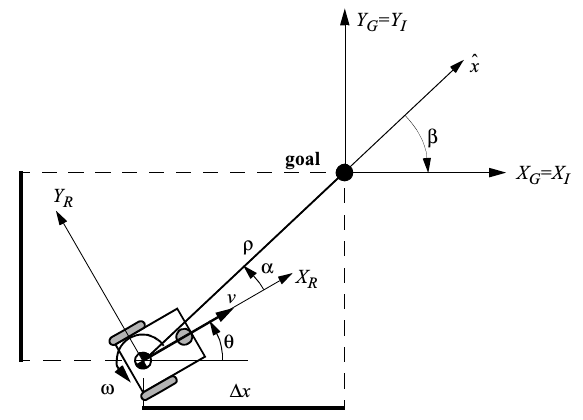
\includegraphics[width=0.60\linewidth]{images/control_polar.png}}
 \captionsetup{font=footnotesize}
 \caption{Configuraci\'on para el control polar donde se muestran la posici\'on del objetivo y los par\'ametros espec\'ificos \cite{siegwart2011introduction}.}
\label{f:controlPolar}
\end{figure}

Una forma alternativa de obtener un control suave de posici\'on y orientaci\'on para un robot es a trav\'es de una ley lineal de control por realimentaci\'on de estados basada en coordenadas polares. Como muestra la Figura ~\ref{f:controlPolar}, las coordenadas polares asociadas con el robot son:
\begin{align*}
\rho &= \sqrt[]{(x_{d} - x)^2 + (y_{d} - y)^2} \\
\alpha &= \text{atan2}(y_{d} - y, x_{d} - x) - \theta \\
\beta &= -\text{atan2}(y_{d} - y, x_{d} - x) + \theta_{d}
\end{align*}
donde $\rho$ representa la distancia desde el robot a la posici\'on de la meta, $\alpha$ y $\beta$ son \'angulos que se utilizan para el error de orientaci\'on. La pose actual del robot es $\x=(x,y,\theta)$, y su pose deseada es $(x_{d},y_{d},\theta_{d})$. En base a estas variables polares, la ley de control que define las velocidades lineales y angulares para lograr la pose deseada es 
\begin{align}
\label{eqn:v}
v &= k_{\rho}\rho \\
\label{eqn:w}
\omega &= k_{\alpha}\alpha + k_{\beta}\beta
\end{align}
donde $k_{\rho}$, $k_{\alpha}$ y $k_{\beta}$ son las ganancias del controlador polar que deben ajustarse adecuadamente para una buena respuesta del sistema. Usando este marco de generaci\'on de movimiento logramos el objetivo tanto en posici\'on como en orientaci\'on.

\section{Navegaci\'on del Robot M\'ovil}

Un robot es un sistema aut\'onomo que puede percibir su entorno y actuar para poder alcanzar sus objetivos. Un robot m\'ovil dentro de un entorno no se encuentra en una ubicaci\'on espec\'ifica, ya que este tiene la capacidad de moverse en su entorno. La principal caracter\'istica que define a un robot aut\'onomo es la capacidad de actuar sobre la base de sus propias decisiones, y no a trav\'es del control de un ser humano \cite{mataric2007robotics}.

La navegaci\'on se define como el proceso o la actividad de determinar con exactitud la posici\'on de uno mismo, planificar y seguir una ruta. En rob\'otica, la navegaci\'on se refiere a la forma en que un robot encuentra su camino en el entorno, es una necesidad y requisito com\'un para casi todos los robots m\'oviles. Esta secci\'on explica los m\'etodos que son empleados en la navegaci\'on aut\'onoma.

\subsection{Campos Potenciales}
La funci\'on potencial m\'as simple es el potencial atractivo y repulsivo. La intuici\'on detr\'as de los campos potenciales es directa: el objetivo atrae al robot mientras los obst\'aculos lo repelen. La suma de estos efectos atrae al robot hacia la meta mientras lo desvía de los obst\'aculos. La funci\'on potencial se puede construir como la suma de potenciales atractivos y repulsivos
%Un campo potencial genera un campo de fuerzas que impulsa al robot hacia la meta evitando obst\'aculos.Esta fuerza tiene dos componentes, un campo de potencial atractivo y un campo de potencial de repulsi\'on
\begin{align}
\label{eqn:potetialField}
U(q) = U_{att}(q) + U_{rep}(q).
\end{align}
\subsubsection{Campo Potencial Atractivo}
Este campo conduce al robot hacia la posici\'on de la meta, suponiendo que hay una pelota determinada alrededor de este objetivo. Es decir, cualquier posici\'on dentro de esta bola se considerar\'a que satisface el objetivo del algoritmo de planificaci\'on. Considere una energ\'ia potencial escalar que depende de la distancia entre la posici\'on actual del robot $\q=(x,y)$ y su posici\'on de objetivo $\text{qgoal}=(\text{xgoal},\text{ygoal})$
\begin{align}
\label{eqn:pot_attr}
U_{att}(q) = \frac{1}{2}\zeta d^{2} (q,q_{goal})
\end{align}
donde $d(a,b)$ es una medida m\'etrica entre dos puntos, y $\zeta$ es un par\'ametro de ajuste que escala el efecto del potencial atractivo. En este caso, usamos la distancia euclidiana como una m\'etrica ya que proporciona buenos resultados experimentales. El gradiente de este campo proporciona un campo vectorial que siempre apunta a la posici\'on de objetivo deseada como:
\begin{align}
\label{eqn:gradient_att}
\nabla U_{att}(q)=\zeta(q-q_{goal}).
\end{align}

\subsubsection{Campo Potencial Repulsivo}
Un potencial repulsivo mantiene al robot alejado de los obst\'aculos. La fuerza de la fuerza de repulsi\'on depende de la proximidad del robot al obst\'aculo. Cuanto m\'as cerca est\'e el robot de un obst\'aculo, m\'as fuerte ser\'a la fuerza de repulsi\'on. Por lo tanto, el potencial repulsivo generalmente se define en t\'erminos de distancia al obst\'aculo m\'as cercano $D(q)$ como 
\begin{equation}
U_{rep}(q) =
\begin{cases}
	\frac{1}{2}\eta(\frac{1}{D(q)} - \frac{1}{Q*})^2, & D(q)\leq Q^* \\
	0, & D(q) > Q^*
\end{cases}
\label{eq:pot_rep}
\end{equation}
donde $Q^* \in \mathbb R$ es una constante que le permite al robot ignorar los obst\'aculos que est\'an lo suficientemente lejos de \'el, y $\eta$ es una ganancia en el gradiente de repulsi\'on. El gradiente es 
\begin{equation}
\nabla U_{rep}(q) =
\begin{cases}
	\eta(\frac{1}{Q^*} - \frac{1}{D})\frac{1}{D^2} \nabla D, & D \leq Q^* \\
	0, & D > Q^*
\end{cases}
\label{eqn:gradient_rep}
\end{equation}
donde la dependencia de $D$ en $q$ ha sido omitida para mayor claridad. Los escalares utilizados para este campo generalmente se determinan por ensayo y error \cite{choset2005principles}.

\section{Movimiento basados en mapas topol\'ogicos (\textit{Roadmap})}

Un \textit{roadmap} es una clase de mapas topol\'ogicos que representan el espacio libre en entornos \cite{choset2005principles}. Los nodos y bordes de un \textit{roadmap} tienen un significado f\'isico. Por ejemplo, un nodo de \textit{roadmap} corresponde a una ubicaci\'on espec\'ifica y un borde corresponde a una ruta entre ubicaciones vecinas.

Los robots usan \textit{roadmaps} de la misma manera que las personas usan los sistemas de carreteras. En lugar de planear todos los caminos laterales posibles hacia un destino, las personas generalmente planean su camino a una red de carreteras. Lo que lleva a la persona desde cerca del inicio hasta cerca de la meta.

Del mismo modo, utilizando un \textit{roadmap}, el robot puede construir una ruta entre dos puntos en un componente conectado del espacio libre del robot encontrando primero una ruta libre de colisiones en el \textit{roadmap}, atravesando el \textit{roadmap} hasta muy pr\'oximo de la meta y luego construyendo una ruta libre de colisiones desde un punto en el \textit{roadmap} hacia la meta. Si el robot conoce el \textit{roadmap}, entonces conoce el entorno. De modo que una forma en que un robot puede explorar un entorno desconocido es confiar en los datos del sensor para construir un \textit{roadmap}.

\section{Movimiento basado en muestreo aleatorio}

%\section{Navegación del Robot Móvil}

%Un robot es un sistema autónomo que puede percibir su entorno y actuar para poder alcanzar sus objetivos. Un robot móvil dentro de un entorno no se encuentra en una ubicación específica, ya que este tiene la capacidad de moverse en su entorno. La principal característica que define a un robot autónomo es la capacidad de actuar sobre la base de sus propias decisiones, y no a través del control de un ser humano \cite{mataric2007robotics}.

%La navegación se define como el proceso o la actividad de determinar con exactitud la posición de uno mismo, planificar y seguir una ruta. En robótica, la navegación se refiere a la forma en que un robot encuentra su camino en el entorno, es una necesidad y requisito común para casi todos los robots móviles.

%La navegación de robots es un campo bastante extenso y se puede dividir en subcategorías para una mejor comprensión de los problemas. Leonard and Durrant-Whyte \cite{leonard1991mobile}, describen brevemente el problema general de la navegación de los robots móviles en tres simples preguntas, cada una refiriendose a una subcategoría:
%\begin{itemize}
%\item[•] \textbf{``¿Dónde estoy?"}\\
%Esta pregunta constituye el problema de localización que se puede expresar como: Un robot se encuentra en una posición desconocida en un entorno para el que tiene un mapa. ``Observa" su posición y, basándose en estas observaciones, debe inferir el lugar o conjunto de lugares en el mapa donde podría ubicarse.
%\item[•] \textbf{``¿A dónde voy?"}\\
%El problema de mapeo consiste en que un robot se encuentra en un entorno desconocido para el cual no tiene un mapa, y al navegar a través de él se habilita la creación de una representación de mapa. El robot debe identificar las características especiales en los puntos de referencia del entorno para reconocer dónde se encuentran los obstáculos.
%\item[•] \textbf{``¿Cómo llego hasta ahí?"}\\
%El problema de la planificación de la ruta es una preocupación general por encontrar rutas que conecten diferentes ubicaciones en un entorno con objetivos específicos y limitaciones.
%\end{itemize}

%La navegación actualmente es un problema difícil y complejo, con muchas soluciones y enfoques diferentes. En \cite{leonard1991mobile} se menciona que el problema no es el proceso de navegación, sino la adquisición de la información y la correlación o correspondencia automática de esa información con algún mapa de navegación, eso hace que el problema de la navegación autónoma sea difícil.
%Un helicóptero es un vehículo volador que utiliza motores de giro rápido para empujar el aire hacia abajo, creando así una fuerza de empuje manteniendo el helicóptero en alto. Los helicóptero convencionales tienen dos rotores. Éstos se pueden disponer como dos rotores coplanares que proporcionan el empuje ascendente, pero que giran en direcciones opuestas (para equilibrar los pares ejercidos sobre el cuerpo del helicóptero)\cite{Gerig2008}.

%Un quadcopter es un helicóptero que tiene cuatro motores con espacios equitativos, por lo general están posicionados en las esquinas de un cuerpo cuadrado. Este tiene 6 grados de libertad (3 de translación y 3 de rotación) y cuatro entradas para la velocidad de los motores.En esta sección de la tesis se explica sobre las ecuaciones matemáticas correspondientes al modelo dinámico del quadcopter. Este modelo esta basado en la teoría de Euler-Lagrange \cite{Bouabdallah2007} y Newton-Euler \cite{Luukkonen2011}, para esta tesis se utilizará la teoría de Newton-Euler.

%\subsection{Campos Potenciales}

%\subsection{Campo Potencial de Atracción}

%\section{Robótica Probabilística}

%Para el desarrollo de esta tesis se utilizó como herramienta los fundamentos de la  Robótica Probabilística, esta basado en el libro de Sebastian Thrun \cite{Thrun2005}.Para que el robot pueda saber sobre el ambiente donde se encuentra, necesita utilizar sensores.Los sensores tienen una limitación en lo que pueden percibir (por ejemplo, el alcance y la resolución). Estos también están sujetos a ruido, lo que desvía las mediciones de los sensores de maneras impredecibles. Este ruido limita la información que se puede extraer de las mediciones del sensor. Los actuadores del robot (por ejemplo,motores) también están sujetos a ruido, lo que introduce incertidumbre. Otra fuente de incertidumbre es causada por el software del robot, que utiliza modelos aproximados del mundo real. Los errores de modelo son una fuente de incertidumbre que a menudo se ha ignorado en los robots. Los robots son sistemas en tiempo real y esto requiere el uso de aproximaciones algorítmicas, pero aumenta la cantidad de incertidumbre aún más.

%Para algunas aplicaciones robóticas (por ejemplo, robots KUKA utilizado en industrias), la incertidumbre es un factor marginal. Dado que los robots están cada vez más desplegados en el mundo abierto, la cuestión de la incertidumbre se ha convertido en un gran desafío para el diseño de robots capaces. La robótica probabilística es un enfoque relativamente nuevo de la robótica que presta atención a la incertidumbre en la percepción y la acción. La incertidumbre se representa explícitamente usando el cálculo de la teoría de la probabilidad. Esto significa que los algoritmos probabilísticos representan la información por distribuciones de probabilidad sobre un espacio. Esto permite representar la ambigüedad y el grado de creencia de una manera matemáticamente correcta. Ahora, los robots pueden tomar decisiones con respecto a la incertidumbre que permanece, o eligieron reducir la incertidumbre si esa es la mejor opción (para esta tesis, exploración).


%\subsection{Estimación del estado recursivo}

%\textbf{Definición 1.} Los ambientes se caracterizan por el estado, que describe todos los aspectos de un robot y el medio ambiente que pueden afectar el futuro. Un estado puede ser un \textit{estado estático}(no cambiante) o un \textit{estado dinámico} (cambiante) en el que ciertas variables de estado tienden a cambiar con el tiempo. Un estado se denomina $x$. El estado en el tiempo $t$ se denota $x_{t}$.

%Las variables del estado son:
%\begin{itemize}
%\item[•] \textit{La pose del robot}: Es la localización y orientación del robot con respecto a un marco global de coordenadas.
%\item[•] \textit{La velocidad del robot}: Es la velocidad para cada pose del robot.
%\item[•] \textit{La ubicación y características de los objetos en el entorno}: Los objetos pueden ser estáticos o dinámicos. Los objetos son modelados como puntos de referencia, cada uno con características distintas y estacionarias que permiten un reconocimiento fiable.
%\end{itemize}

%Una de las ideas de la robótica probabilística es la estimación del estado a partir de los datos del sensor, pero los sensores solo observan una parte de la información total y sus mediciones se ven afectadas por el ruido. Por ende la estimación del estado intenta recuperar las variables de estado a partir de los datos. En lugar de calcular un único estado, este calcula una distribución probabilística sobre los posibles estados en el mundo real.Esta distribución probabilística es llamada \textit{belief} y es descrita en la siguiente página.

%\textbf{Definición 2.} La estimación de estados se encargan del problema de estimar las varibales de estado a partir de los datos de los sensores que no son directamente observables, pero se puede inferir. Una distribución probabilística se calcula sobre los posibles estados del mundo real.

%Un robot puede interactuar con su entorno influyendo en el estado de su entorno a través de sus actuadores (acciones de control), o puede recopilar información sobre el estado a través de sus sensores (mediciones del sensor en el ambiente).

%\textbf{Definición 3.} El conjunto de todas las mediciones adquiridas desde el tiempo $t_{1}$ hasta el tiempo $t_{2}$, para $t_{1} \leqslant t_{2}$ es igual a:
%\begin{equation}
%z_{t_{1}:t_{2}} = z_{t_{1}}, z_{t_{1} + 1}, z_{t_{1} + 2}, \ldots , z_{t_{2}}
%\end{equation}
 
%\textbf{Definición 4.} El conjunto de todos los datos de control desde el tiempo $t_{1}$ hasta el tiempo $t_{2}$, para $t_{1} \leqslant t_{2}$ es igual a:
%\begin{equation}
%u_{t_{1}:t_{2}} = u_{t_{1}},u_{t_{1} + 1}, u_{t_{1} + 2}, \ldots , u_{t_{2}}
%\end{equation}

%Los datos de control transmiten información relativa al cambio de estado. Por ejemplo, establecer la velocidad de un robot a 1 $m/s$, sugiere que la nueva posición del robot después de 2 segundos está aproximadamente 2 metros por delante de su posición antes de ejecutar el comando.
%Generalmente, las mediciones proporcionan información sobre el estado del ambiente, aumentando el conocimiento del robot. El problema de esta información es que el movimiento del robot tiende a inducir una pérdida de conocimiento debido al ruido inherente en el accionamiento del robot.
%La evolución del estado y las mediciones se realizan mediante leyes probabilísticas.El estado ~$x_{t}$ es generado estocásticamente desde el estado ~$x_{t-1}$. Cuando se dice que el estado ~$x_{t}$ es completo, implica que se sabe ~$x_{t-1}$.Las mediciones pasadas y los controles no transmiten ninguna información con respecto al estado ~$x_{t}$. Esta suposición se conoce como \textit{Markov Assumption} y se expresa de la siguiente forma:
%\begin{equation}
%\label{eqn:markov-assumption1}
%p(x_{t}\mid x_{0:t-1}, z_{1:t-1}, u_{1:t}) = p(x_{t}\mid x_{t-1}, u_{t})
%\end{equation}
%donde $p(x_{t}\mid x_{t-1}, u_{t})$ es llamada probabilidad de transición de estado y especifica cómo evoluciona el estado ambiental a lo largo del tiempo en función del control del robot $u_{t}$.  

%\textbf{Definición 5.} \textit{Markov Assumption} establece que los datos pasados y futuros son independientes si se conoce el estado actual $x_{t}$. Esto significa que los valores en cualquier estado son influenciados solamente por los valores del estado que lo precedieron directamente.
%El proceso por el cual se modelan las mediciones se expresa:
%\begin{equation}
%\label{eqn:markov-assumption2}
%p(z_{t}\mid x_{0:t}, z_{1:t-1}, u_{1:t}) = p (z_{t}\mid x_{t})
%\end{equation}
%donde $p(z_{t}\mid x_{t})$ is llamado probabilidad de medición y especifica cómo se generan las mediciones a partir del estado del ambiente $x_{t}$.

%Otra idea de la robótica probabilística es \textit{belief}, que refleja el conocimiento del robot sobre el estado del mundo real. Las distribuciones de creencias son probabilidades posteriores sobre variables de estado condicionadas a los datos disponibles. \textit{Markov Assumption} implica que la creencia actual es suficiente para representar la historia pasada del robot. El \textit{belief} sobre las variables de estado se expresa como $bel(x_{t})$:
%\begin{equation}
%bel(x_{t}) = p(x_{t}\mid z_{1:t}, u_{1:t})
%\end{equation}

%Se puede realizar una predicción del estado en el tiempo $t$ antes de incorporar una medición. Esta predicción es usada en el contexto del filtrado probabilístico y es denotado como:
%\begin{equation}
%\overline{bel}(x_{t}) = p(x_{t}\mid z_{1:t-1}, u_{1:t})
%\end{equation}
%esta ecuación predice el estado en el tiempo ~$t$ basado en el estado anterior, antes de incorporar la medida en el tiempo ~$t$.

%\textbf{Definición 6.} \textit{Belief} refleja el conocimiento del robot sobre el estado del entorno, a través de distribuciones de probabilidad condicional. \textit{Belief} sobre la variable de estado $x_{t}$ es denotado por $bel(x_{t})$.


%\subsection{Algoritmos}

%El algoritmo más general para calcular los \textit{belief} es el filtro de Bayes. La entrada del algoritmo es el \textit{belief} $bel$ en el instante $t-1$, el control $u_{t}$ más reciente y la medición $z_{t}$. En primer lugar, se calcula una predicción para la nueva creencia basada en el control $u_{t}$ (la medición es ignorada):
%\begin{equation}
%\label{eqn:BF-prediction}
%\overline{bel}(x_{t}) = \int p(x_{t}\mid u_{t},x_{t-1})bel(x_{t-1})dx_{t-1}.
%\end{equation}
%El segundo paso de los filtros de bayes es la medición actualizada:
%\begin{equation}
%\label{eqn:BF-measurement}
%bel(x_{t}) = \eta p(z_{t}\mid x_{t})\overline{bel}(x_{t})
%\end{equation}
%donde $\eta$ es una constante de normalización para asegurar una probabilidad válida. Ahora,$bel(x_{t})$ es el \textit{belief} del robot sobre el estado, después los datos de medición y control se usan para mejorar el conocimiento del robot. Ambos pasos del algoritmo se realizan recursivamente para todas las mediciones y comandos de control.

%La familia más popular de los estimadores de estado recursivos son los filtros gaussianos. Los filtros gaussianos representan el \textit{belief} mediante distribuciones normales multivariadas (aproximadas por una función gaussiana). 
%\begin{equation}
%p(x)= det(2\pi\Sigma)^{-\frac{1}{2}} exp\{-\frac{1}{2}(x-\mu)^{T}\Sigma^{-1}(x-\mu)\}
%\end{equation}
%La función densidad (probabilidad) sobre el espacio de estado $x$ se caracteriza por dos parámetros: la media $\mu$ y la covarianza $\Sigma$.
%Los gaussianos son unimodales y tienen un único máximo. Sin embargo, esto es característico para muchos problemas de seguimiento, donde el posterior se centra alrededor del estado verdadero con un cierto margen de incertidumbre.
%Con el fin de implementar los filtros descritos anteriormente, se requiere dos componentes adicionales. En la sección 2.2.3,se describe el modelo de movimiento y en la sección 2.2.4 se describe el modelo de medición.


%\subsection{Modelo de Movimiento}

%Los modelos de movimiento probabilísticos describen la relación entre la pose anterior con la actual, también lo controles (comandos) emitidos por una distribución de probabilidad. Esto es llamado como la probabilidad de transición de estado. La probabilidad de transición de estado juega un papel esencial en la etapa de predicción del filtro de Bayes.

%\textbf{Definición 7.} Un modelo de movimiento probabilístico define la transición de estado entre dos etapas de tiempo consecutivas $t-1$ y $t$ después de que se ha llevado a cabo una acción de control $u_{t}$. Se expresa por la distribución posterior $p(x_{t}\mid x_{t-1}, u_{t})$.

%Existe dos modelos de movimiento probabilístico complementarios que son el modelo de movimiento de velocidad y el modelo de movimiento de odometría. El modelo de movimiento de velocidad asume que un robot es controlado a través de dos velocidades: una velocidad de rotación $\omega_{t}$ y la velocidad de traslación $v_{t}$.
%\begin{equation}
%u_{t} = \begin{pmatrix}
%v_{t} \\
%\omega_{t}
%\end{pmatrix}
%\end{equation}

%La probabilidad $p(x_{t}\mid x_{t-1}, u_{t})$ se puede calcular con algoritmos que se pueden encontrar en \cite{Thrun2005}. El modelo de movimiento de odometría asume que uno tiene acceso a la información de los encoders de la rueda. En la práctica, los modelos de odometría tienden a ser más precisos, porque la mayoría de los robots no ejecutan el comando de velocidad con el nivel de precisión que se obtiene midiendo la odometría. Técnicamente, las lecturas de odometría no son controles porque se reciben después de ejecutar un comando. Sin embargo, el uso de lecturas de odometría como controles da como resultado una formulación más sencilla del problema de estimación.

%Ambos modelos no se pueden aplicar a los drones. Por ejemplo, un quadcopter es controlado a través de sus ángulos de rotación (pitch, roll y yaw). Se requiere una conversión entre ángulos y velocidades para usar el modelo de movimiento de velocidad para un quadcopter. Para los robots de tierra, la odometría puede obtenerse mediante la integración de la lectura de los encoders de cada rueda, pero un quadcopter no tiene contacto con el suelo, por ende no se puede realizar odometría. En su lugar, se utilizan diferentes fuentes de información para obtener información de odometría. Por ejemplo, el quadcopter de esta tesis utilizará un sensor láser para obtener esta información.

%\subsection{Modelo de Medición}

%Los modelos probabilísticos de medición describen la relación entre los estados del mundo real $x_{t}$ y cómo se realiza un lectura del sensor $z_{t}$ (observación). Basándose en el estado estimado del mundo real $x_{t}$, se genera un \textit{belief} sobre las posibles mediciones. El ruido en las mediciones del sensor se modela explícitamente, inherente a la incertidumbre de los sensores del robot. Para expresar el proceso de generación de mediciones, se requiere una especificación del entorno. Un mapa $m$ del entorno es una lista de objetos y ubicaciones:
%\begin{equation}
%m =\{m_{1}, m_{2}, \ldots, m_{N}\}
%\end{equation}
%donde $N$ es el total de números de objetos en el ambiente.Los mapas suelen ser mapas basados en características o mapas basados en la ubicación. Los mapas basados en ubicación son volumétricos y ofrecen una etiqueta para cualquier ubicación. Los mapas basados en funciones sólo describen la forma del entorno en ubicaciones específicas, que son comúnmente objetos. Los mapas basados en características son más populares debido a que la representación hace más fácil ajustar la posición de los objetos.

%\textbf{Definición 8.} Un modelo de sensor probabilístico describe la relación entre un estado del mundo real $x_{t}$ y la lectura del sensor $z_{t}$ dado un modelo del ambiente $m$ en forma de una distribución posterior $p(z_{t}\mid x_{t},m)$.

%\subsection{Localización}
%El problema de la localización de un robot es estimar la posición (estado) del robot en relación con el mapa del entorno. La localización es un componente importante para la navegación de un robot, junto con la percepción, la cognición y el control de movimiento.

%Cuando un robot se mueve en un entorno conocido y comienza en una ubicación conocida, puede realizar un seguimiento de su ubicación mediante la integración de estimaciones de posición local (por ejemplo, odometría). Debido a la incertidumbre de estas estimaciones locales, la incertidumbre de la ubicación absoluta del robot aumenta con el tiempo. Con el fin de reducir la incertidumbre, el robot tiene que recuperar su posición absoluta localizándose en relación con un mapa. Para ello, el robot utiliza sus sensores para hacer observaciones de su entorno y relaciona estas observaciones con un mapa del medio ambiente.

%Un enfoque probabilístico de la localización utiliza el \textit{belief} para representar la localización global estimada. De nuevo, actualizar la posición del robot implica dos pasos. El primer paso se denomina actualización de predicción. El robot utiliza su estado en el tiempo $t-1$ y los datos del control $u_{t}$ para predecir su estado en el instante $t$. Este paso de predicción aumenta la incertidumbre sobre el estado del robot. El segundo paso se llama actualización de la percepción. En este paso, el robot utiliza la información de sus sensores para corregir la posición estimada durante la fase de predicción, reduciendo la incertidumbre sobre el estado del robot. 
%\subsection{Mapeo y Localización simultánea (SLAM)}
%Un problema mucho más difícil de la localización es cuando no conoces el mapa del ambiente. En este caso, la información del sensor del robot se utiliza para recuperar la trayectoria del robot y construir un mapa del entorno.
%Este problema se llama Mapeo y Localización simultánea (\textit{SLAM}). Una solución a este problema haría  un robot auténticamente autónomo. \textit{SLAM} es un problema difícil porque tanto el camino estimado como el mapa construido son afectados por el ruido. Ambos se vuelven cada vez más inexactos durante el viaje. Sin embargo, cuando se revisa un lugar que ha sido mapeado, se puede reducir la incertidumbre.
%Este proceso se denomina cierre de bucle. Además, se puede optimizar el mapa después de que se detecta un evento de cierre de bucle.
%\subsubsection{Técnicas de Solución}
%En la práctica, no es posible calcular analíticamente el \textit{belief} del robot (probabilidades posteriores). Por lo tanto, existen varias técnicas de aproximación. Esta sección describe las técnicas de solución más populares para los problemas de \textit{SLAM}.

%Las técnicas de solución se pueden dividir en dos ramas principales de la representación del \textit{belief}: \textit{single-hypothesis belief} y \textit{multi-hypothesis belief}. \textbf{Single-hypothesis trackers} representan la creencia de un solo estado del mundo real. Esta estimación esta asociada por una medida de certidumbre (o varianza), que permite al rastreador ampliar o estrechar la región estimada en el espacio de estado. La principal ventaja de la representación \textit{single-hypothesis} es la ausencia de la ambigüedad, simplificando la toma de decisiones en el nivel cognitivo del robot (por ejemplo, la planificación de la trayectoria). Debido a la ausencia de ambigüedad, los rastreadores no modelan adecuadamente las ambigüedades.

%\textbf{Multi-hypothesis trackers} representa el \textit{belief} no solo como un único estado del mundo real, sino como un conjunto posiblemente infinito de estados. La principal ventaja de la representación \textit{multi-hypothesis} es que el robot puede mantener explícitamente la incertidumbre respecto a sus estado. Esto permite a un robot creer en múltiples poses simultáneamente, permitiendo al robot rastrear y rechazar diferentes hipótesis independientemente. Una de las principales desventajas de una representación \textit{multi-hypothesis} implica la toma de decisiones. Si el robot representa su posición como un conjunto de puntos, se vuelve menos obvio calcular la mejor acción.

%Además, las técnicas de solución se pueden dividir en dos ramas de las limitaciones de tiempo: \textit{online computing} y \textit{offline computing}. Las técnicas \textbf{online} resuelven un problema en tiempo real y deben garantizar la respuesta dentro de estrictas restricciones de tiempo. Una ventaja de las técnicas en línea es la capacidad de utilizar la respuesta como entrada para la toma de decisiones (por ejemplo, la navegación), que es esencial para los robots autónomos. Debido a las estrictas restricciones de tiempo, se puede realizar una cantidad limitada de cálculos, lo que limita la complejidad de las técnicas de solución.

%Las técnicas \textbf{offline} tienen restricciones de tiempo menos estrictas, lo que permite una mayor complejidad. Por ejemplo, se pueden realizar mejoras adicionales que serían demasiado lentas para las técnicas en línea. Una de las principales desventajas de las técnicas \textit{offline} implica la toma de decisiones. Debido a que una respuesta no está disponible en tiempo real, el robot tiene que esperar o tomar una decisión sin incorporar la respuesta.

%\textbf{Filtro de Kalman (KF)}

%La técnica más popular para implementar un filtro de Bayes es el Filtro de Kalman (1960) \cite{kalman1960new}, es mayormente utilizado para mejorar la navegación de vehículos. El filtro tiene una representación de \textit{single-hypothesis belief} y se puede realizar en tiempo real. El filtro de Kalman se basa en la suposición de que el sistema es lineal y tanto el modelo de movimiento como el modelo de medición se ven afectados por el ruido gaussiano.El \textit{belief} en el tiempo $t$ está representada por una distribución gaussiana multivariable definida por su media $\mu_{t}$ y la covarianza $\Sigma_{t}$. Esto significa que $x_{t}$ del filtro de Bayes (ecuaciones \ref{eqn:BF-prediction} y \ref{eqn:BF-measurement}) ha sido reemplazado por $\mu_{t}$ y $\Sigma_{t}$.

%El filtro de Kalman asume que el sistema es lineal: la transición de estado $A$ (ecuación \ref{eqn:markov-assumption1}), el modelo de movimiento $B$ y el modelo del sensor $C$ (ecuación \ref{eqn:markov-assumption2}) son funciones lineales únicamente dependiendo del estado $x$ o del comando de control $u$, más un modelo de ruido gaussiano $Q$:
%\begin{equation}
%\label{eqn: Kalman Filter}
%\begin{matrix}
%\textrm{\textbf{Predicción}}\\
%\overline{\mu}_{t} &= &A_{t}\mu_{t-1} + B_{t} u_{t} &\textrm{estimación de la media a-priori}\\
%\overline{\Sigma}_{t} &= &A_{t}\Sigma_{t-1} A_{t}^{T} + R_{t} &\textrm{estimación de la covarianza a-priori}\\
%\textrm{\textbf{Actualización}}\\
%K_{t} &= &\overline{\Sigma}_{t}C_{t}^{T}(C_{t}\overline{\Sigma}_{t}C_{t}^{T} + Q_{t})^{-1} &\textrm{Ganancia de Kalman}\\
%\mu_{t} &= &\overline{\mu}_{t} + K_{t}(z_{t} - C_{t}\overline{\mu}_{t}) &\textrm{actualización estimación de estado (a posteriori)}\\
%\Sigma_{t} &= &(I - K_{t}C_{t})\overline{\Sigma}_{t} &\textrm{actualización estimación de la covarianza (a posteriori)}\\
%\end{matrix}
%\end{equation}

%El filtro de Kalman representa el \textit{belief} $bel(x_{t})$ en el tiempo $t$ por la media $\mu_{t}$ y la covarianza $\Sigma_{t}$. Cuando se recibe una medición, se predice una nueva creencia $bel(x_{t})$ basada en el \textit{belief} anterior $bel(x_{t-1})$, los datos de control $u_{t}$ y tanto el modelo de transición de estado como el modelo de movimiento. Este \textit{belief} predecida describe el estado más probable $\overline{\mu}_{t}$ en el tiempo $t$ y la covarianza $\overline{\Sigma}_{t}$. La medición todavía no está incluida, porque es un \textit{belief} que se predice. El paso de la actualización cambia el \textit{belief} predecido ($\overline{\mu}_{t},\overline{\Sigma}_{t}$) en el \textit{belief} deseado ($\mu_{t},\Sigma_{t}$), incorporando la medición $z_{t}$. La ganancia de Kalman $K_{t}$ especifica el grado que la medición se incorpora en la nueva estimación del estado. El concepto clave utilizado para filtración de kalman es la innovación, que es la diferencia entre la medición real $z_{t}$ y la medición esperada $C_{t}\overline{\mu}_{t}$, que se deriva del estado predecido. Una medida $z_{t}$ que está lejos de la medida predecida, es menos fiable, por lo tanto es menos probable que se incorpore en la nueva estimación del estado.

%El filtro de Kalman estándar requiere un sistema lineal, que no es suficiente para describir muchos problemas de la vida real. Por lo tanto, se han propuesto variaciones del algoritmo original que pueden hacer frente a diferentes niveles de no-linealidad. Estas variaciones se aproximan a los modelos de movimiento y medición de forma que tiendan a ser lineales.

%\textbf{Filtro Extendido de Kalman}

%El filtro extendido de Kalman es una variante del filtro de Kalman que puede utilizarse para sistemas no lineales. Este intenta aproximar los modelos de movimiento y de medición no lineales a sistemas lineales. La probabilidad de transición de estado y las probabilidades de medición son representadas por las funciones no lineales $g$ y $h$:
%\begin{equation}
%\begin{matrix}
%x_{t} &= & g(u_{t},x_{t-1})\\
%z_{t} &= & h(x_{t}) + \delta_{t}
%\end{matrix}
%\end{equation}
%estas funciones reemplazan las matrices de operación A,B y C del filtro de Kalman (ecuación \ref{eqn: Kalman Filter}).

%La idea clave de la aproximación de Filtro Extendido de Kalman se llama linealización. Una aproximación lineal de primer orden de Taylor se calcula a la medida de la creencia actual (Gaussiana), resultando una función lineal. Proyectar la creencia gaussiana a través de la aproximación lineal da como resultado una densidad gaussiana.
%\begin{equation}
%\begin{matrix}
%\textrm{\textbf{Predicción}}\\
%\overline{\mu}_{t} &= &g(u_{t},\mu_{t-1}) &\textrm{estimación de la media a-priori}\\
%\overline{\Sigma}_{t} &= &G_{t}\Sigma_{t-1}G_{t}^T + R_{t} &\textrm{estimación de la covarianza a-priori}\\
%\textrm{\textbf{Actualización}}\\
%K_{t} &= &\overline{\Sigma}_{t}H_{t}^{T}(H_{t}\overline{\Sigma}_{t}H_{t}^{T} + Q_{t})^{-1} &\textrm{Ganancia de Kalman}\\
%\mu_{t} &= &\overline{\mu}_{t} + K_{t}(z_{t} - h(\overline{\mu}_{t})) &\textrm{actualización estimación de estado (a posteriori)}\\
%\Sigma_{t} &= &(I - K_{t}H_{t})\overline{\Sigma}_{t} &\textrm{actualización estimación de la covarianza (a posteriori)}.\\
%\end{matrix}
%\end{equation}

